\documentclass[a4paper,10pt]{article}
\usepackage[utf8]{inputenc}

\usepackage{graphicx}

%opening
\title{Task 3: RNN for many to many prediction}
\author{Matthias}


\begin{document}

\maketitle

\section{approach}

Parameters: $n_1$ the length of learning curves for training, $n_2$ the length of learning curves for predictions

\begin{itemize}
 \item Train an RNN on learning curves of length $n_1$, at each step using the next step as target.
 \item Provide the configuration at the first step only (alternative: at each step).
 \item Prediction: feed the first $n_2$ steps of the learning curve into the RNN to predict step $n_2 + 1$.
 \item Then append the predicted step to the learning curve and feed it into the RNN to predict step $n_2 + 2$.
 \item Repeat until step 40.
\end{itemize}


\section{expectations}

\begin{itemize}
 \item increasing $n_1$ should generalise much better
 \item risk of propagating errors (erronous prediction at step $k$ is fed into the network to predict step $k+1$)
 \item increasing $n_2$ should reduce this risk
 \item not sure if predictions for steps $k > n_1$ make sense, when all training sequences only had length $n_1$
\end{itemize}


\section{first insights}

\begin{itemize}
 \item small $n_1$ or small $n_2$ are both problematic
 \item if the RNN predicts that the test error increases at step $k$, it increases all the following steps (sometimes even leading to final predictions greater than 1)
 \item overall it seems a promising method, since training and validation losses get below 0.001 (but that's for the prediction of the first $n_1$ steps
  of a sequence, not for the final test error!)
 \item when training on all steps ($n_1 = 40$) and $n_2 = 20$, the test loss for the prediction of the final training error is 0.001403 (after training only 10 epochs),
  but we should choose $n_1 \in \{5, 10, 20\}$
\end{itemize}

The following plot shows 10 predicted curves (using the test set of the first CV fold), resulting from training on whole sequences (all 40 steps), and prediction using the first 20 steps
from the sequence (steps 21 to 40 are predicted by the RNN and then fed back into it to predict the following step):\\
green = true curve, red = prediction

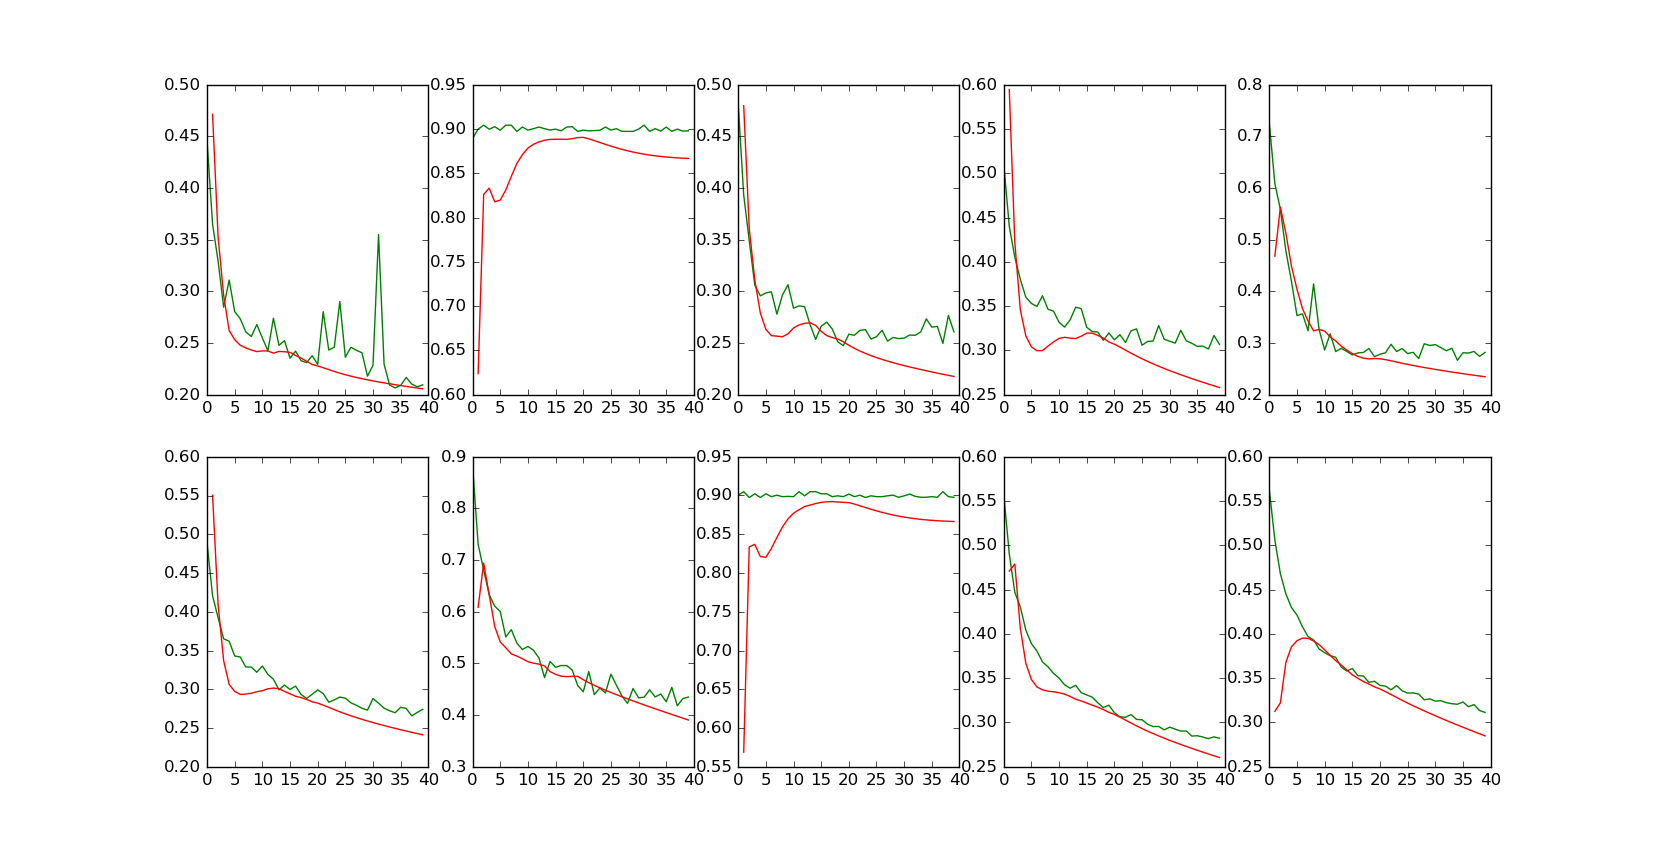
\includegraphics[width=\textwidth]{../../figures/lstm_many2many_39train-steps_20pred-steps}

So far, the RNN seems to underestimate the error in each step.


\section{first results}

The evaluation is made on 1 fold only, training for 200 epochs.

\begin{tabular}{|c|c|c|c|c|c|}
 \hline
 $n_{train}$ & $n_{test}$ & training loss & validation loss & final test E40 loss & best test E40 loss (@epoch) \\
 \hline
 5 & 5 & 0.000929 & 0.001588 & 0.145444 & 0.077837 (@149) \\
 10 & 10 & 0.000646 & 0.001357 & 0.044646 & 0.005268 (@109) \\
 20 & 20 & 0.000535 & 0.000684 & 0.009755 & 0.003154 (@99) \\
 \hline
\end{tabular}


\section{example curves}

Training and prediction on 5 steps, after training for 150 epochs:

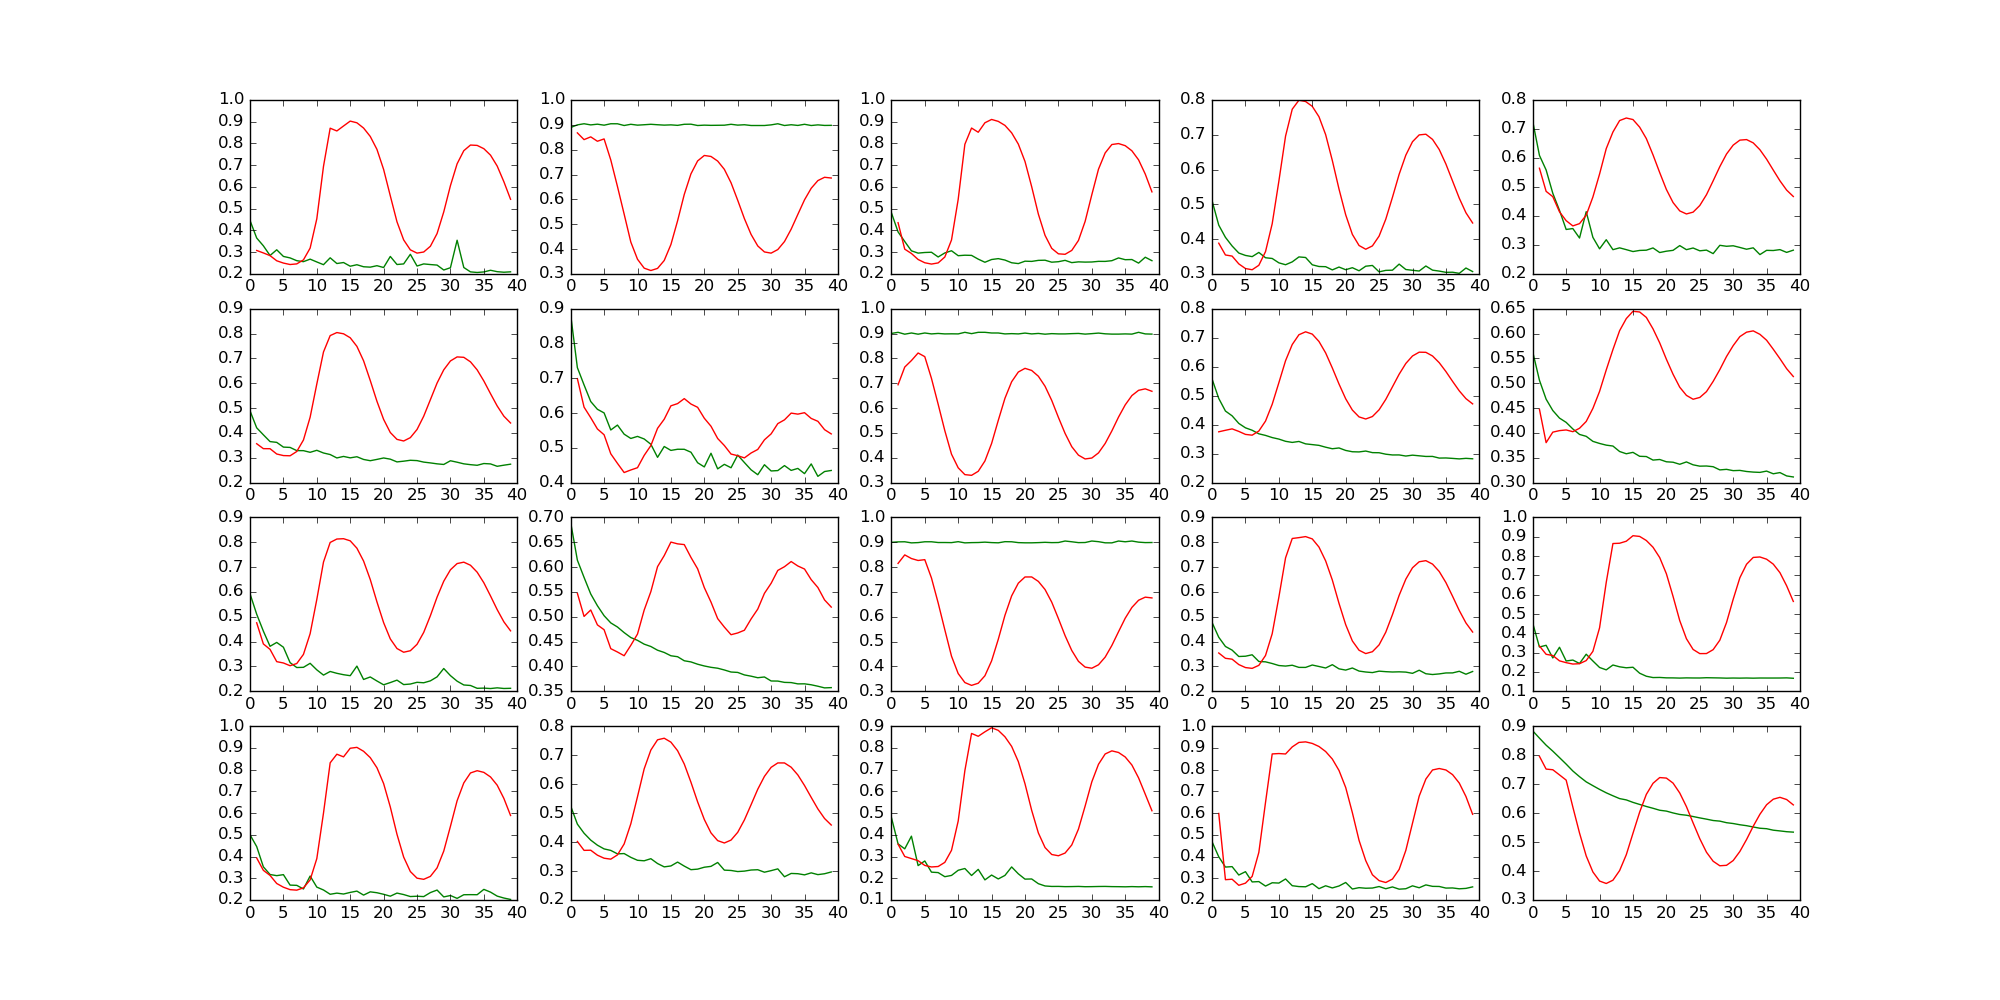
\includegraphics[width=\textwidth]{../../figures/LSTM_m2m_5_steps_epoch_149}

Training and prediction on 5 steps, after training for 200 epochs:

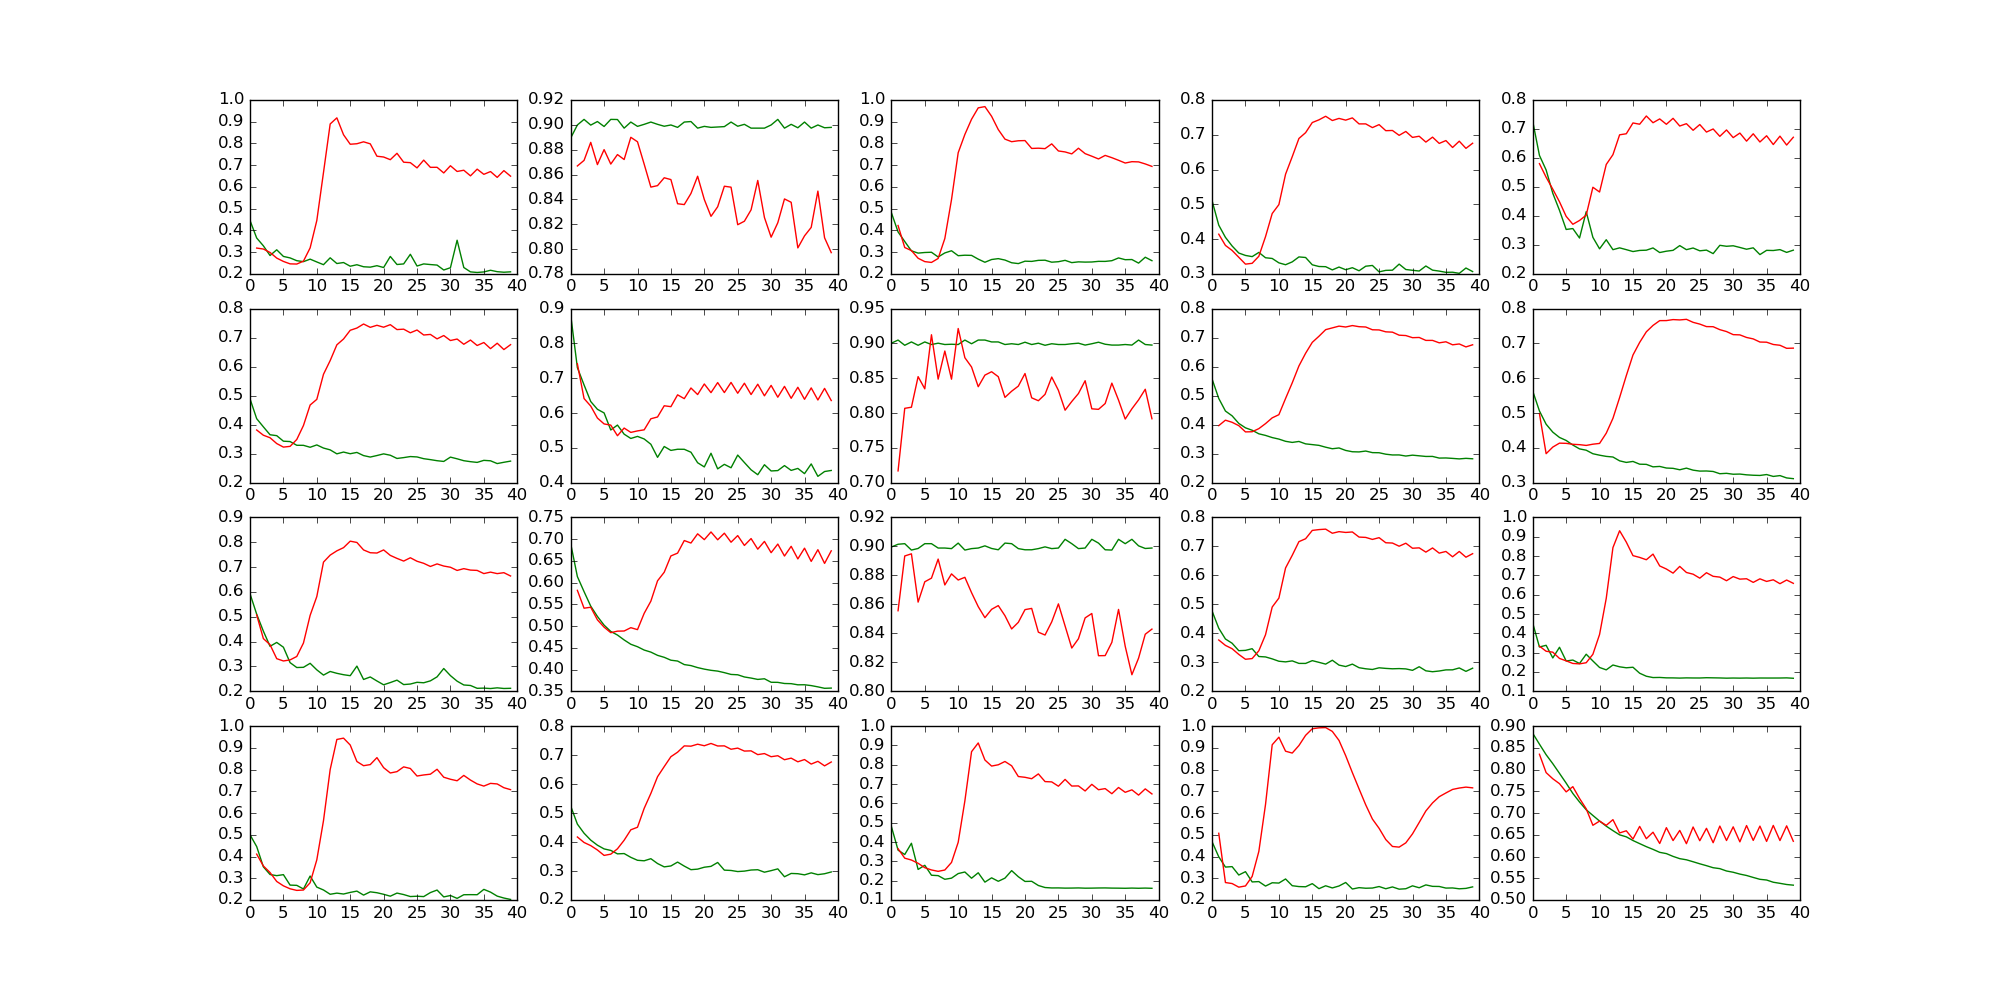
\includegraphics[width=\textwidth]{../../figures/LSTM_m2m_5_steps_epoch_199}

Training and prediction on 10 steps, after training for 110 epochs:

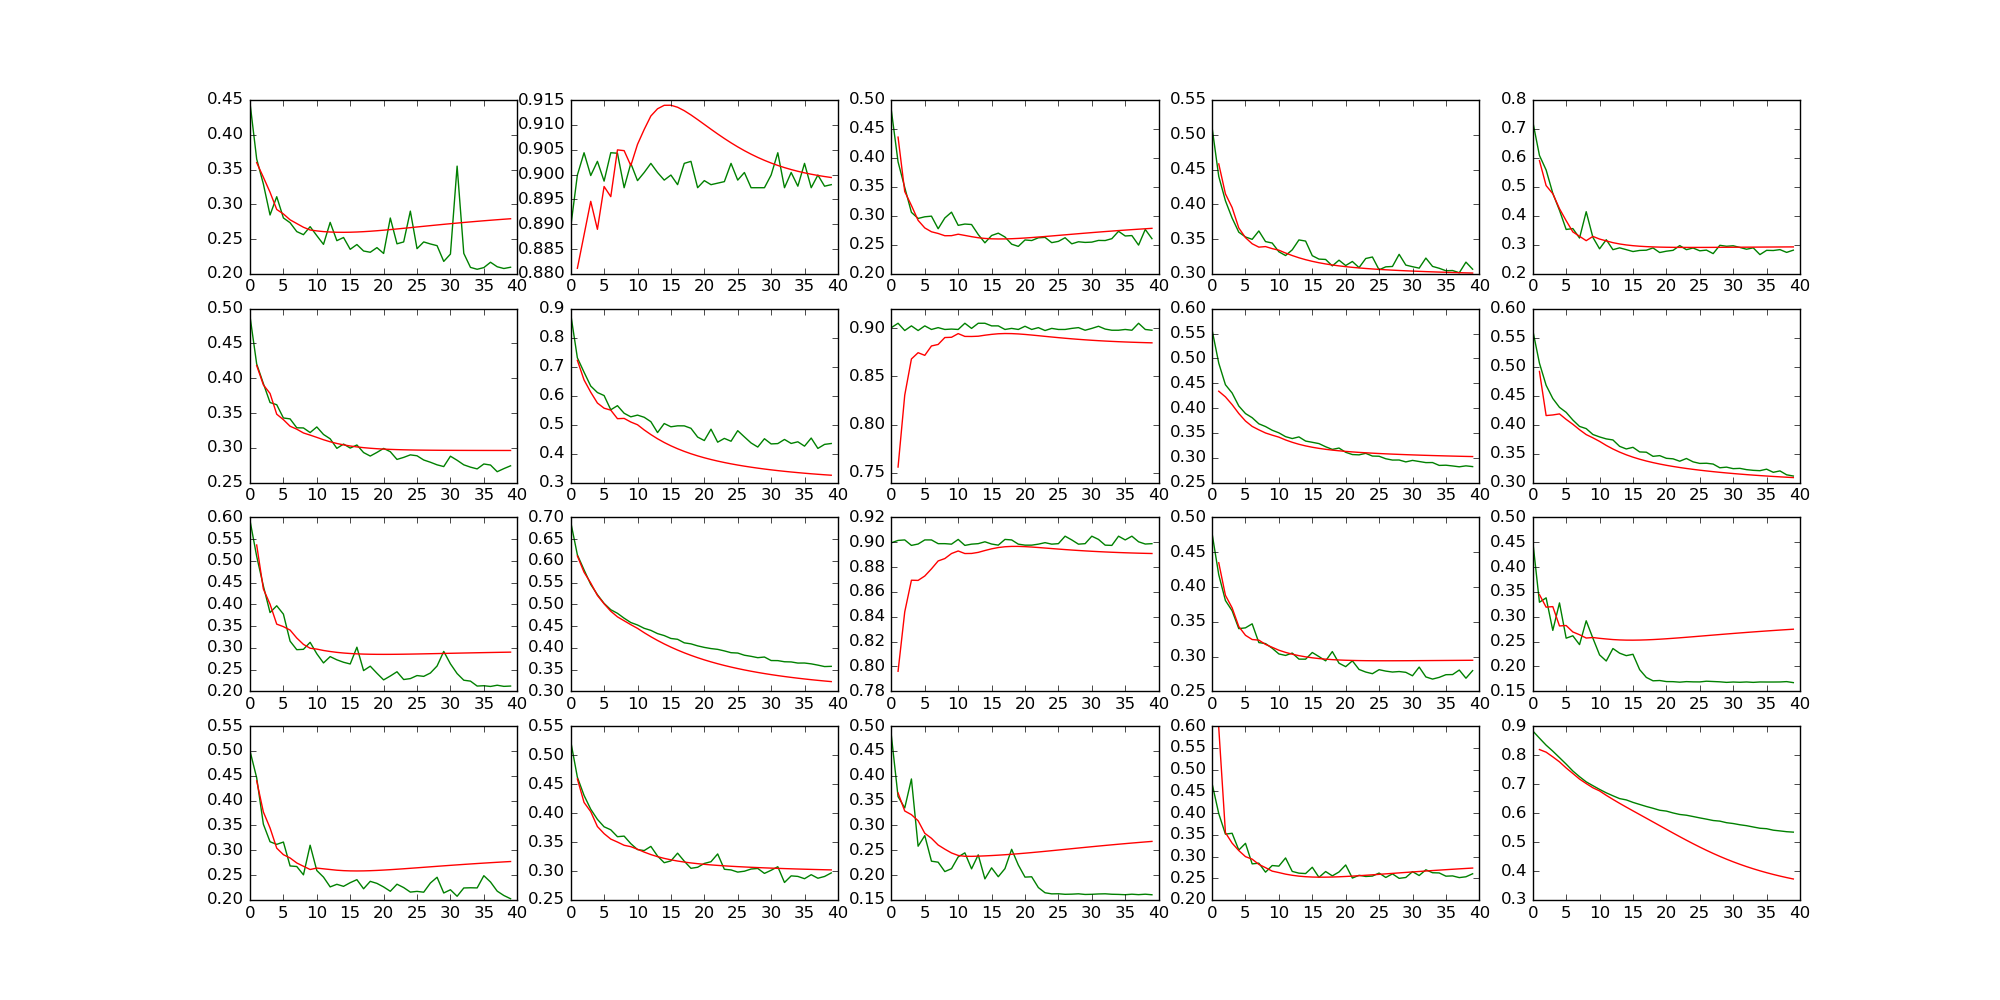
\includegraphics[width=\textwidth]{../../figures/LSTM_m2m_10_steps_epoch_109}

Training and prediction on 10 steps, after training for 200 epochs:

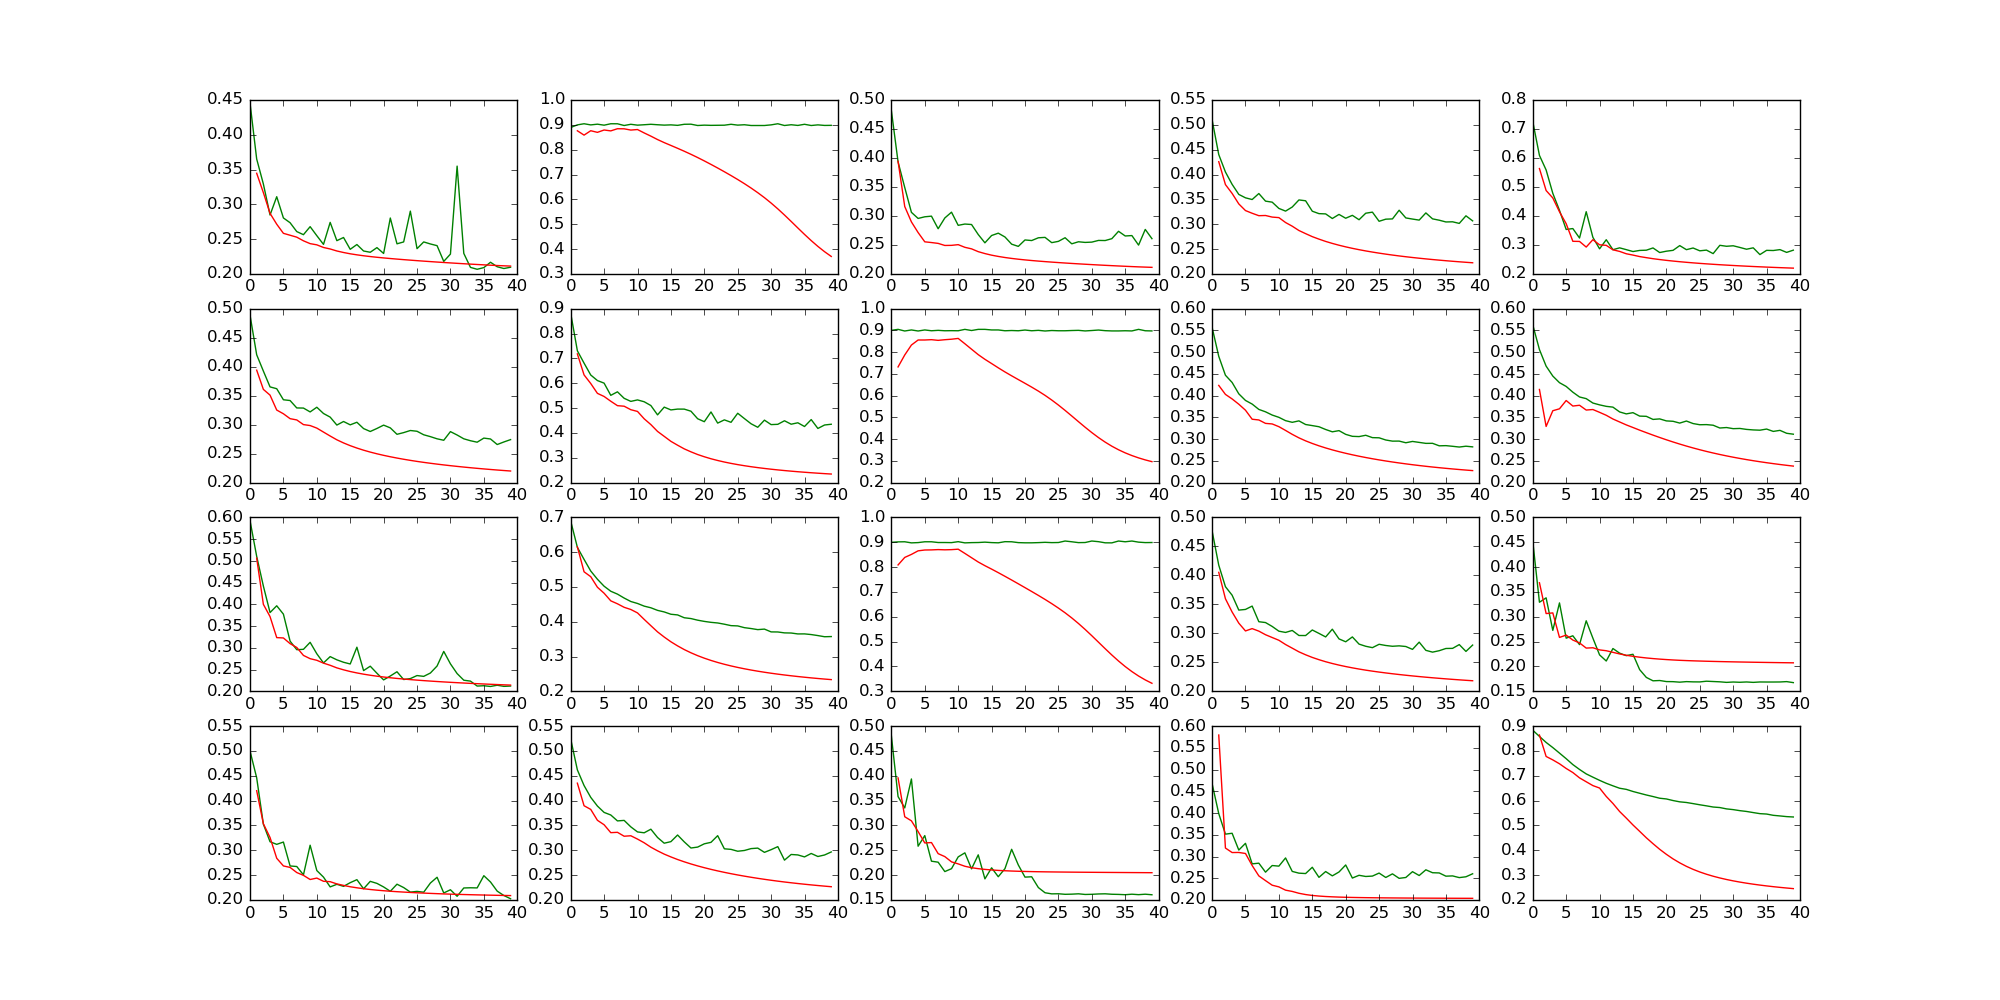
\includegraphics[width=\textwidth]{../../figures/LSTM_m2m_10_steps_epoch_199}

Training and prediction on 20 steps, after training for 100 epochs:

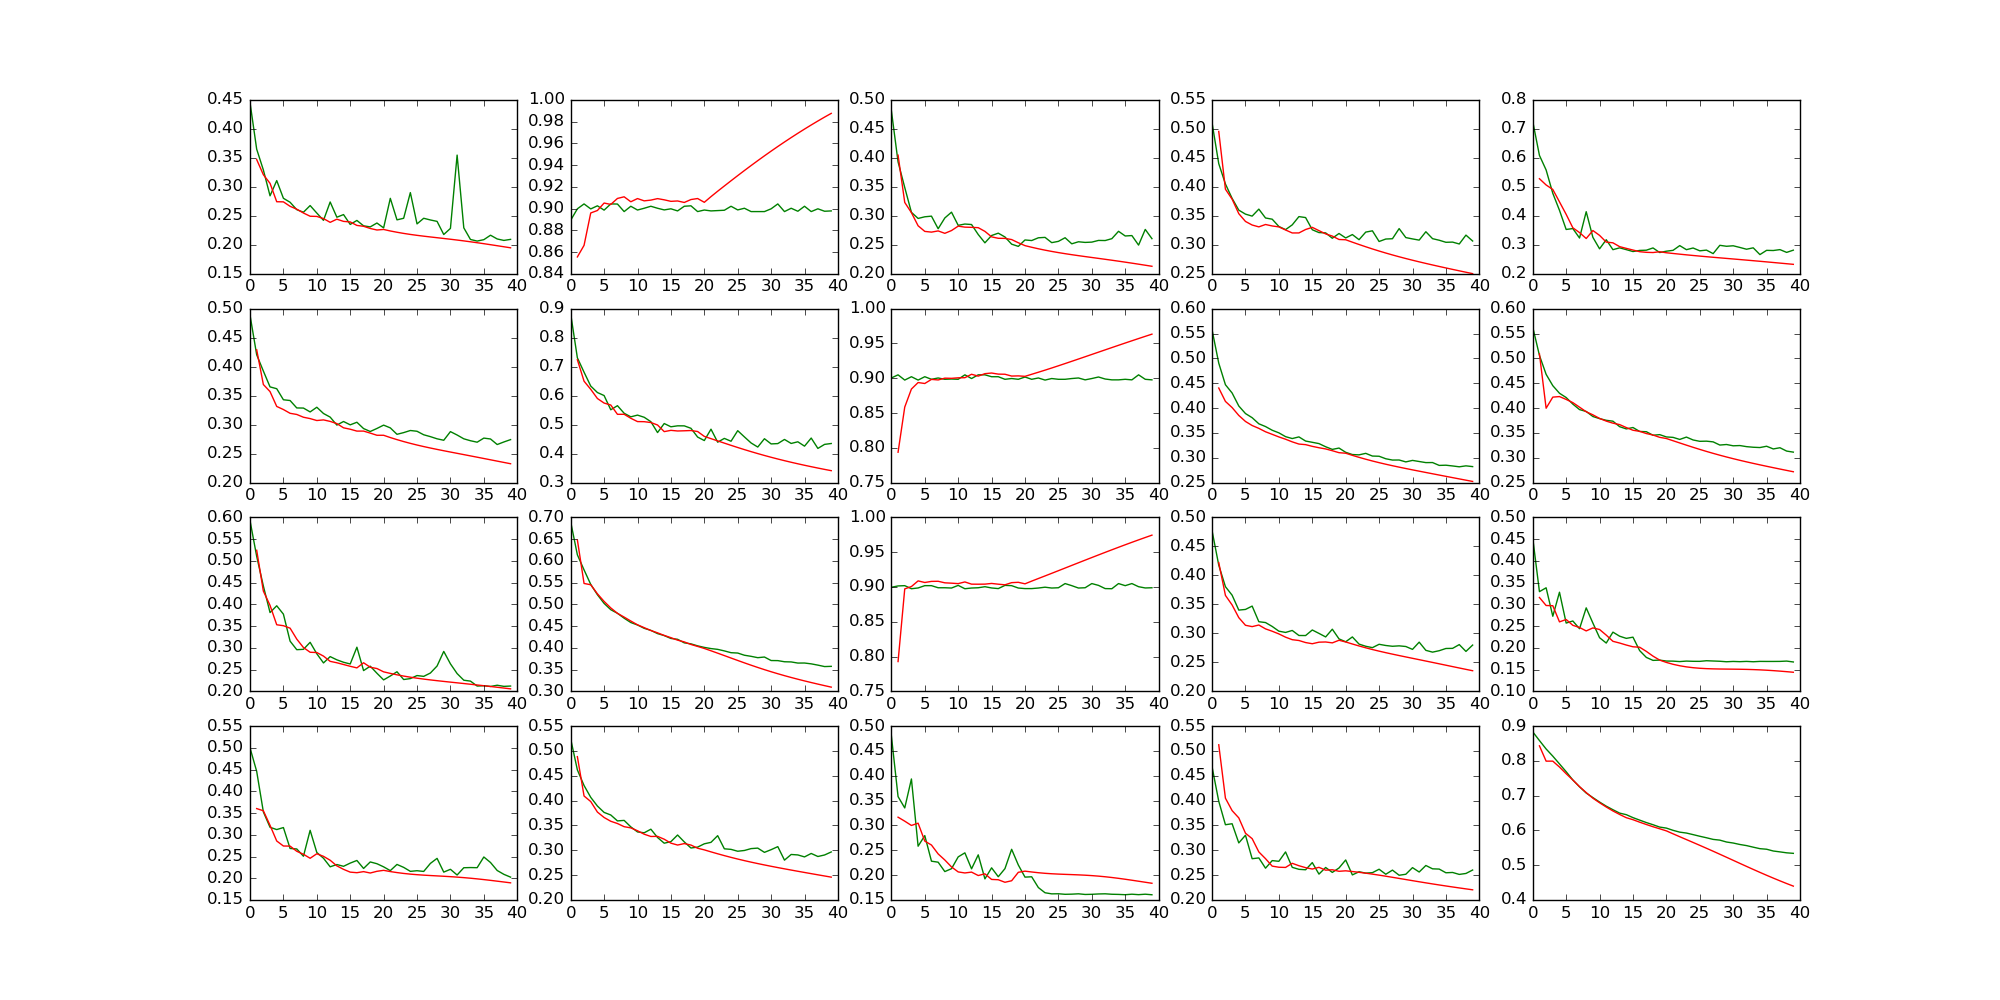
\includegraphics[width=\textwidth]{../../figures/LSTM_m2m_20_steps_epoch_99}

Training and prediction on 20 steps, after training for 200 epochs:

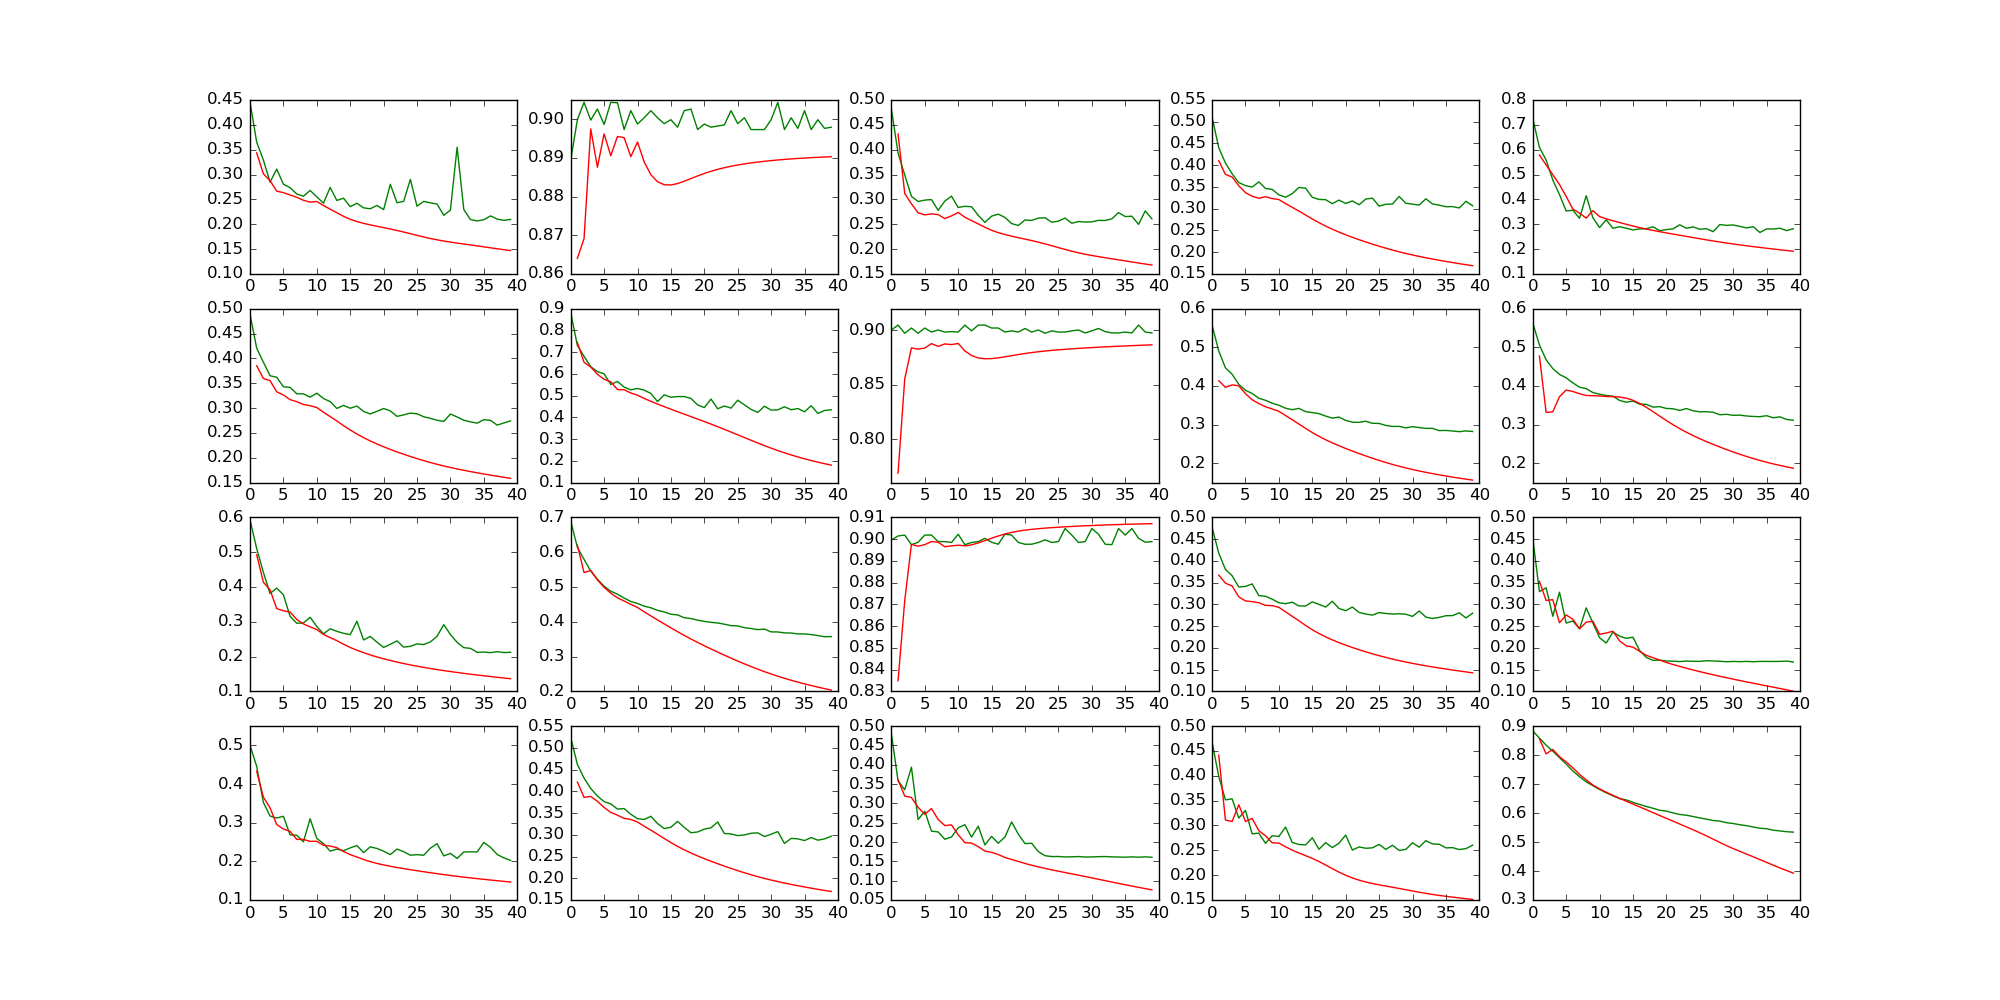
\includegraphics[width=\textwidth]{../../figures/LSTM_m2m_20_steps_epoch_199}

\end{document}
